\documentclass[12pt]{article}
%% arXiv paper template by Flip Tanedo
%% last updated: Dec 2016



%%%%%%%%%%%%%%%%%%%%%%%%%%%%%
%%%  THE USUAL PACKAGES  %%%%
%%%%%%%%%%%%%%%%%%%%%%%%%%%%%

\usepackage{amsmath}
\usepackage{amssymb}
\usepackage{amsfonts}
\usepackage{graphicx}
\usepackage{xcolor}
\usepackage{nopageno}
\usepackage{enumerate}
\usepackage{parskip}
\usepackage{framed}

\usepackage{sectsty}
\sectionfont{\large}
% \renewcommand{\thesection}{}
% \renewcommand{\thesubsection}{\arabic{subsection}}

%%%%%%%%%%%%%%%%%%%%%%%%%%%%%%%%%%%%%%%%%%%%%%%
%%%  PAGE FORMATTING and (RE)NEW COMMANDS  %%%%
%%%%%%%%%%%%%%%%%%%%%%%%%%%%%%%%%%%%%%%%%%%%%%%

\usepackage[margin=2cm]{geometry}   % reasonable margins

\graphicspath{{figures/}}	        % set directory for figures

% for capitalized things
\newcommand\acro[1]{{\small {#1}}}

\numberwithin{equation}{section}    % set equation numbering
\renewcommand{\tilde}{\widetilde}   % tilde over characters
\renewcommand{\vec}[1]{\mathbf{#1}} % vectors are boldface

\newcommand{\dbar}{d\mkern-6mu\mathchar'26}    % for d/2pi
\newcommand{\ket}[1]{\left|#1\right\rangle}    % <#1|
\newcommand{\bra}[1]{\left\langle#1\right|}    % |#1>
\newcommand{\Xmark}{\text{\sffamily X}}        % cross out

\let\olditemize\itemize
\renewcommand{\itemize}{
  \olditemize
  \setlength{\itemsep}{1pt}
  \setlength{\parskip}{0pt}
  \setlength{\parsep}{0pt}
}


% Commands for temporary comments
\newcommand{\comment}[2]{\textcolor{red}{[\textbf{#1} #2]}}
\newcommand{\flip}[1]{{\color{red} [\textbf{Flip}: {#1}]}}
\newcommand{\email}[1]{\texttt{\href{mailto:#1}{#1}}}

\newenvironment{institutions}[1][2em]{\begin{list}{}{\setlength\leftmargin{#1}\setlength\rightmargin{#1}}\item[]}{\end{list}}


\usepackage{fancyhdr}		% to put preprint number



% Commands for listings package
%\usepackage{listings}      % \begin{lstlisting}, for code
%
% \lstset{basicstyle=\ttfamily\footnotesize,breaklines=true}
%    sets style to small true-type



%%%%%%%%%%%%%%%%%%%
%%%  HYPERREF  %%%%
%%%%%%%%%%%%%%%%%%%

%% This package has to be at the end; can lead to conflicts
\usepackage{microtype}
\usepackage[
	colorlinks=true,
	citecolor=black,
	linkcolor=black,
	urlcolor=green!50!black,
	hypertexnames=false]{hyperref}





\begin{document}


\begin{center}

    {\Large \textsc{Long HW 1}:
    \textbf{Vectors, Matrices, and Indices}}
    
\end{center}

\vskip .4cm

\noindent
\begin{tabular*}{\textwidth}{rl}
	\textsc{Course:}& Physics 017, \emph{Linear Algebra for Physics} (S2022)
	\\
	\textsc{Instructor:}& Prof. Flip Tanedo (\email{flip.tanedo@ucr.edu})
	\\
	\textsc{Due by:}& \textbf{Thursday}, April 7
\end{tabular*}

\noindent
This is the `long' assignment assigned every two weeks. You should aim to complete it within two weeks because you'll have new assignments by then, but the formal due date is two weeks + two days. Your explainer video assignment will be to present one of these problems.

Part of the challenge of the `long' homework may be to figure out exactly what is being asked. Be sure to use the beginning of lecture (or office hours) to ask early when you are confused. Sometimes we are \emph{intentionally} using jargon that you may not be familiar with in order to encourage you to ask and/or look things up.\footnote{Sometimes this is just because the professor is absent minded about what students know and do not yet know.} A good mantra that was once told to the professor when he was a student: \emph{There are no stupid questions. Only stupid students who do not ask questions when they are confused.}

\section*{Background}

In this problem set we use the abstract bra-ket notation. Perhaps you are used to writing vectors as $\overrightarrow{v}$ or $\vec{v}$. In our abstract notation, vectors are called `kets' and are written $|v\rangle$. This is just notation, there is no math or science involved in this. 

The usual basis vectors for $\mathbb{R}^N$ are $\hat{\vec{x}}$, $\hat{\vec{y}}$, etc. Sometimes we write them as $\hat{\vec{e}}_1$, $\hat{\vec{e}}_2$, etc. In other words,
\begin{align}
	\hat{\vec{x}} &= \hat{\vec{e}}_1 = 
	\begin{pmatrix}
		1\\0\\ \vdots
	\end{pmatrix}
	&
	\hat{\vec{y}} &= \hat{\vec{e}}_2 = 
	\begin{pmatrix}
		0\\1\\ \vdots
	\end{pmatrix} \ ,
\end{align}
and so forth. The basis kets are typically written as $|1\rangle = \hat{\vec{x}} = \hat{\vec{e}_1}$ and similarly for $|2\rangle$, $|3\rangle$, and so forth. The notation has its pros and cons---you will soon appreciate them in this class---but since it is new, we should get used to it. A vector $|v\rangle$ is expanded in basis kets as
\begin{align}
	|v\rangle = v^1|1\rangle + v^2 |2\rangle + \cdots \ .
\end{align}
The components $v^i$ can be arranged as a column of numbers if you want to recover the expression for vectors.



\section{Matrices as Vectors}\label{sec:matrixspace}

Here's something that sounds totally wacky. We can define a vector space of matrices. Here is a basis for $2\times 2$ real matrices:
\begin{align}
	|1\rangle &= 
	\begin{pmatrix}
		1 & 0 \\ 0 & 0
	\end{pmatrix}
	&
	|2\rangle &= 
	\begin{pmatrix}
		0 & 1 \\ 0 & 0
	\end{pmatrix}
	&
	|3\rangle &= 
	\begin{pmatrix}
		0 & 0 \\ 1 & 0
	\end{pmatrix}
	&
	|4\rangle &= 
	\begin{pmatrix}
		0 & 0 \\ 0 & 1
	\end{pmatrix} \ .
	\label{eq:matrix:basis}
\end{align}

\subsection{Writing a matrix as a vector}

What are the vector components $v^i$ of the following matrix? 
\begin{align}
	|v\rangle& = 
		\begin{pmatrix}
			1 & 4\\
			2 & 7
		\end{pmatrix} \ .
\end{align}

{\small \textsc{Comment:} we say \emph{matrix}, but really this object is a $2\times 2$ array of numbers that should be understood as a funny-looking vector space.}

\subsection{Writing a vector as a matrix}

Write the following vector, $|w\rangle$ as a $2\times 2$ matrix using the basis \eqref{eq:matrix:basis}:
\begin{align}
	|w\rangle = \pi |1\rangle + e|2\rangle - 2 |3\rangle + 2.4|4\rangle \ .
\end{align}

\subsection{Changing Basis}

Here's a new basis for the vector space of $2\times 2$ real matrices:
\begin{align}
	|1'\rangle &= 
	\begin{pmatrix}
		1 & 0 \\ 0 & 1
	\end{pmatrix}
	&
	|2'\rangle &= 
	\begin{pmatrix}
		1 & 0 \\ 0 & -1
	\end{pmatrix}
	&
	|3'\rangle &= 
	\begin{pmatrix}
		0 & 1 \\ 1 & 0
	\end{pmatrix}
	&
	|4'\rangle &= 
	\begin{pmatrix}
		0 & 1 \\ -1 & 0
	\end{pmatrix} \ .
	\label{eq:matrix:basis:prime}
\end{align}
What are the components $(v')^i$ and $(w')^i$ of the vectors $|v\rangle$ and $|w\rangle$ in this basis? These are defined by, for example:
\begin{align}
	|v\rangle = (v')^1|1'\rangle + (v')^2|2'\rangle + (v')^3|3'\rangle + (v')^4|4'\rangle \ .
\end{align}
Make sure to explain how you do this; your explanation is more valuable than the final answer. 

\subsection{Linear Independence}

Consider the \textbf{subspace} of the vector space of $2\times 2$ matrices that is \textbf{spanned} by only the first three basis vectors in \eqref{eq:matrix:basis}. This is the three-dimensional vector space whose vectors can all be written in the form
\begin{align}
	|v\rangle = v^1|1\rangle + v^2 |2\rangle + v^3 |3\rangle \ .
\end{align}
Let's call this subspace $V_3$. We can analogously define a subspace $V'_3$ formed out of linear combinations of first three basis vectors in \eqref{eq:matrix:basis:prime}. These are composed of vectors of the form
\begin{align}
	|v\rangle = (v')^1|1'\rangle + (v')^2 |2'\rangle + (v')^3 |3'\rangle \ .
\end{align}
Please write down one example of a vector from the `full' vector space of $2\times 2$ real matrices that live in each four regions of the following Venn diagram:

\begin{center}
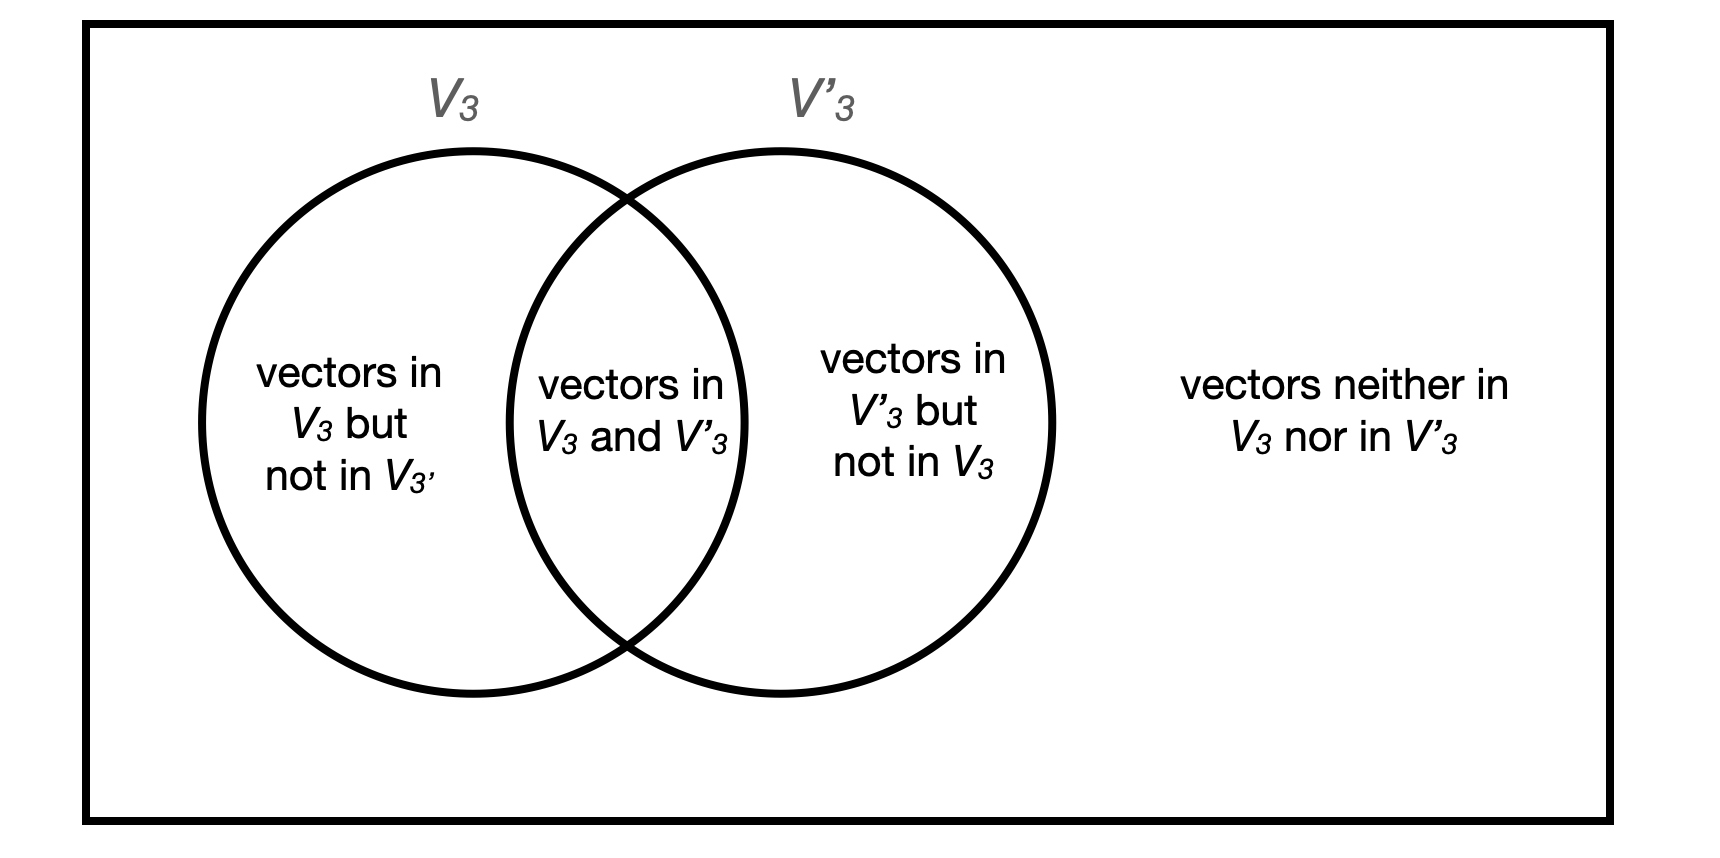
\includegraphics[width=.5\textwidth]{figures/HW1b_vectors.png}
\end{center}

\section{The Gram--Schmidt Procedure}

In microbiology, a Gram-positive bacteria are those that have a peptidoglycan cell wall layer\footnote{\url{https://en.wikipedia.org/wiki/Gram-positive_bacteria}}. This problem has nothing to do with that. In linear algebra, the Gram--Schmidt procedure is a way to take a set of linearly independent vectors and produce an \textbf{orthonormal} basis out of them.

In the first parts of this problem, please be sure to draw your pictures carefully and use them to explain the process.


\subsection{Two linearly independent vectors}

Consider the two-dimensional vector space $\mathbb{R}^2.$ Suppose we have the linearly independent vectors,\footnote{For familiarity we're using column notation. You could also write $|v\rangle = 4|\hat{x}\rangle + 1|\hat{y}\rangle$. They mean the same thing.}
\begin{align}
	|v\rangle &= 
	\begin{pmatrix}
		4\\1
	\end{pmatrix}
	&
	|w\rangle = 
	\begin{pmatrix}
		1\\-2
	\end{pmatrix} \ .
\end{align}
Here we have written the vectors in the `standard basis' so that the first component is the length in the $x$-direction and the second component is the length in the $y$-direction. Please draw these two vectors.

\subsection{Creating the first orthonormal basis vector}\label{sec:orthonormal}
Define $|\hat{v}\rangle$ to be the unit vector that is parallel to $|v\rangle$. What are the components of $|\hat{v}\rangle$ in the standard basis? These are the components $\hat v^i$ such that
\begin{align}
	|\hat v\rangle = 
	\hat v^1 
	\begin{pmatrix}
	1 \\ 0	
	\end{pmatrix}
	+ 
	\hat v^2 
	\begin{pmatrix}
	0 \\ 1
	\end{pmatrix} \ .
\end{align}
\textsc{Hint~1}: what is the condition for a vector to be a unit vector? (Please do not say that the vector is large.\footnote{\url{https://knowyourmeme.com/memes/absolute-unit}}) What does this condition imply on the components $\hat v^i$? 

\textsc{Hint~2}: What does it mean for two vectors to be parallel? What does this condition imply on the components $\hat v^i$? 

Please draw the vector $|\hat v\rangle$ along with the vectors $|v\rangle$ and $|w \rangle$. We will use $\hat v\rangle$ as one of our new basis vectors. Hooray.

\subsection{Orthogonal and non-orthogonal pieces}\label{sec:orthogonal}

Our next goal is to find $|\hat w_\perp\rangle$, a second basis vector that is (1) orthogonal to $|\hat v\rangle$ and (2) it is a unit vector. Let us do the first part. The goal is to separate $|w \rangle$ into two pieces:
\begin{align}
	|w_\rangle &= |w_\parallel\rangle + |w_\perp\rangle \ ,
	\label{eq:w:perp:parallel}
\end{align}
where $|w_\parallel\rangle$ is parallel to $|v\rangle$ and $|w_\perp\rangle$ is perpendicular to $v$. Find the components $w_\parallel^i$ and $w_\perp^i$ of these vectors.

\textsc{Hint:} The parallel component is related to the dot product of $|w\rangle$ and $|\hat v\rangle$, which we may write as $\langle w,\hat v\rangle \equiv \vec{w}\cdot\hat{\vec{v}}$. Figure out this relation and write $|w_\parallel\rangle$ with respect to $\langle w, \hat{v}\rangle$ and $|\hat{v}\rangle$. Then use  \eqref{eq:w:perp:parallel} to figure out $|w_\perp\rangle$. 

\subsection{Normalize}

We now know that $|w_\perp\rangle$ is perpendicular to $|\hat v \rangle$. It is not yet normalized. Follow the steps in Part~\ref{sec:orthonormal} to define a normalized unit vector $|\hat w_\perp \rangle$ that is parallel to $|w_\perp\rangle$. Draw $|\hat w_\perp\rangle$, $|\hat v\rangle$, $|v\rangle$, and $|w\rangle$ together. Confirm from the drawing that we have successfully derived an orthonormal basis: $|\hat v\rangle$ and $|\hat w_\perp\rangle$.

\subsection{What if we went the other way around?}

Would you end up with the same set of basis vectors if you started the Gram--Schmidt process with $|w\rangle$ first? Explain why or why not; your explanation must include a picture illustrating the result.

\subsection{More dimensions}
Mo' dimensions, mo' problems\footnote{The Notorious B.I.G.\ taught us \emph{I don't know what they want from me /
It's like the more money we come across /
The more problems we see}. Often in physics the more dimensions there are the more subtle the system becomes. There is at least one exception in quantum field theory where physicists often go to $d+\varepsilon$ dimensions... this is like saying we go from 4 dimensions to 4.0001 dimensions. Crazy, right? This is called dimensional regularization and it is used as a trick to tame some unruly integrals. By the way, 4 dimensions = 3 spatial dimensions and 1 time dimension. There are some cases where we work with spacetimes with two time dimensions, but physical space is always some subspace with only one time dimension. A famous example is Anti de-Sitter space, which is at the core of what string theorists call the hologrpahic principle and is the kind of thing illustrated in some of M.C.~Escher's most famous prints.}?
How would the Gram--Schmidt process change if the vector space is three-dimensional? You end up repeating the steps for each additional. Please explain what happens in Part~\ref{sec:orthogonal} when you have to separate the third vector into perpendicular and parallel parts. 

\textsc{Commentary:} For the second vector, you just needed parts perpendicular and parallel to the first vector. For the third vector, you now have a choice between projections onto the first and the second vector. 

\subsection{Orthonormal matrix space}

Recall the vector space of $2\times 2$ real matrices and the unusual basis in \eqref{eq:matrix:basis:prime}. Define a dot product (or inner product or metric... these are all the same thing) between vectors in this space as follows:
\begin{align}
	\langle v,w\rangle = \vec{v}\cdot \vec{w} = \text{Tr}(\vec v \vec w) \ .
	\label{eq:matrix:dot}
\end{align}
In other words: let $|v\rangle$ and $|w\rangle$ be vectors that are $2\times 2$ matrices. The inner product is the trace of the product of these matrices. For example:
\begin{align}
	\left\langle
	\begin{pmatrix}
		1 & 3\\
		2 & 1
	\end{pmatrix}
	\, , \, 
	\begin{pmatrix}
		2 & 1\\
		0 & -1
	\end{pmatrix}
	\right\rangle
	= 
	\text{Tr}\left[\begin{pmatrix}
		1 & 3\\
		2 & 1
	\end{pmatrix}
	\begin{pmatrix}
		2 & 1\\
		0 & -1
	\end{pmatrix}\right]
	=
	\text{Tr}
	\begin{pmatrix}
		2 & -2 \\ 4 & 1
	\end{pmatrix}
	= 
	3 \ .
\end{align}
Take a moment to appreciate why this could be a good definition for an inner product. Confirm that $\langle v,w\rangle = \langle w,v\rangle$. Also confirm that $\langle v+w, t\rangle = \langle v,t\rangle + \langle w, t\rangle$. 

Apply the Gram--Schmidt procedure to the basis in \eqref{eq:matrix:basis:prime} to create an orthonormal basis.

\textsc{Hint:} Doing a four-dimensional Gram--Schmidt is kind of annoying. However, the basis in \eqref{eq:matrix:basis:prime} naturally splits into two pairs that are mutually orthogonal. Start by showing that the diagonal matrices and the off-diagonal matrices are orthogonal to each other with respect to the inner product \eqref{eq:matrix:dot}.






\section{Rotations}

% Image from \texttt{memegenerator.net}\footnote{\url{https://memegenerator.net/instance/86179034/dodgeball-patches-if-you-can-rotate-a-vector-you-can-rotate-a-tensor}}
% \begin{center}
% 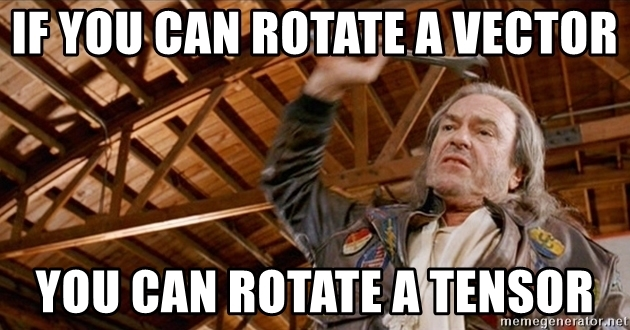
\includegraphics[width=.5\textwidth]{figures/if-you-can-rotate-a-vector-you-can-rotate-a-tensor.jpg}
% \end{center}

\subsection{Rotations and inverse rotations in Euclidean space}

In $\mathbb{R}^2$, one can perform a clockwise rotation by angle $\theta$ on a vector by multiplying the vector by the rotation matrix:
\begin{align}
	R(\theta) & = 
	\begin{pmatrix}
		R^1_{\phantom{1}1} & R^1_{\phantom{1}2}
		\\
		R^2_{\phantom{21}1} & R^2_{\phantom{2}2}
	\end{pmatrix}
	&
	R^1_{\phantom{1}1} &= R^1_{\phantom{1}1} = \cos\theta
	&
	R^1_{\phantom{1}2} &= - R^2_{\phantom{2}1} = \sin \theta \ .
\end{align}
In column vector notation, write out the rotation by angle $\theta$ of a vector $\vec{v}$ with components
\begin{align}
	\vec{v} = \begin{pmatrix}
		v^1 \\ v^2
	\end{pmatrix} \ .
\end{align}

\subsection{Passive transformations}

There's a subtle point that always pops up with rotations. Are we rotating the \emph{vector} (as we did above) or are we rotating the \emph{coordinate system} (basis vectors)?  Let $\hat{\vec{e}}_1$ and $\hat{\vec{e}}_2$ be the standard unit vectors in the $x$ and $y$-directions,
\begin{align}
	\hat{\vec{e}}_1 &= 
	\begin{pmatrix}
		1\\0
	\end{pmatrix}
	&
	\hat{\vec{e}}_1 &= 
	\begin{pmatrix}
		0\\1
	\end{pmatrix} \ .
\end{align}
Define a new pair of basis vectors by rotating these basis vectors:
\begin{align}
	\hat{\vec{e}}_1' &= R(\theta) \hat{\vec{e}}_1 & 
	\hat{\vec{e}}_2' &= R(\theta) \hat{\vec{e}}_2 \ .
\end{align}
It should be obvious\footnote{In this class, `obvious' means: if it is not immediately clear to you, ask about this right away because there is a certain way of seeing things that you want to be able to appreciate. We will always use `obvious' this way, so don't be intimidated if something `obvious' is not clear. It only means that you should ask about how to make this idea clear.} that the new basis is orthonormal. Write out new basis vectors as column vectors.

\subsection{Active versus passive}

Rotating the vector $\vec{v}\to R(\theta)\vec{v}$ is called an \textbf{active transformation}. Rotating the basis vectors $\hat{\vec{e}}_i\to R(\theta) \hat{\vec{e}}_i$ is called a \textbf{passive transformation}. Show that an active transformation on $\vec{v}$ by angle $\theta$ is the same as a passive transformation on $\vec{v}$ by an angle $-\theta$.

\textsc{Hint}: use $\sin(-\theta) = -\sin\theta$. 


\subsection{Inverse Rotation}

What are the components of $R^{-1}(\theta)$, the inverse transformation of the rotation by angle $\theta$? Show that this satisfies $R^{-1}(\theta)R(\theta) = R(\theta)R^{-1}(\theta) = 1$, the unit matrix.


\subsection{Exponentiation of a matrix}\label{sec:exponentiation}

Recall that the exponential of a number $x$ is defined by its Taylor expansion,
\begin{align}
	e^{x} = 1 + x + \frac{1}{2!}x^2 + \frac{1}{3!} x^3 + \cdots .
\end{align}
One can define the exponentiation of a matrix $A$ in the same way:
\begin{align}
	e^{A} = 1 + A + \frac{1}{2!}A^2 + \frac{1}{3!} A^3 + \cdots ,
\end{align}
where here $A^n$ is understood to mean matrix multiplication. Show the following relation:
\begin{align}
	e^{i \theta T} &= R(\theta) 
	&
	T &= \begin{pmatrix}
		0 & 1 \\ -1 & 0
	\end{pmatrix}\ .
\end{align}
Note that $\theta$ is just some real number. 

\textsc{Hint}: work out the first few terms explicitly. You should notice a pattern between the even powers and the odd powers. Remember what the Taylor expansions for sine and cosine look like. 

\textsc{Comment}: The matrix $T$ is special, it is called the \textbf{generator} of rotations. The theory of continuous symmetries (Lie groups) is built on the idea of generators for symmetry transformations. This idea finds a killer application in quantum mechanics.




% inner product

% rotating a matrix, rotating a vector, rotating an inner product

% if you can rotate a vector, you can rotate a matrix. 

% order of terms.

% exponentiation

\appendix	

\section{Extra Credit: Complex numbers as vector spaces}

It turns out that complex numbers are a two-dimensional vector space. The complex numbers $\mathbb{C}$ differs from $\mathbb{R}^2$ because it has an added rule called a \textbf{complex structure}. This is basically the rule that $i^2 = -1$. The rotation matrix from Part~\ref{sec:exponentiation} comes in handy, as well as the vector space of matrices in Problem~\ref{sec:matrixspace}. This problem shows the nice connection between complex numbers and rotations.\footnote{The reason why these two are connected lies in the following cryptic statement: both are representations of the Abelian group, $U(1)$.} 

\subsection{Complex Arithmetic}
A complex number is usually written $z = a+ib$. It has a real component $a$ and an imaginary component $b$, where both $a$ and $b$ are real numbers. Another way to write this is as a vector $|z\rangle = a|1\rangle + b|i\rangle$, where the basis elements are
\begin{align}
	|1\rangle &=
	\begin{pmatrix}
		1 & 0 \\ 0 & 1
	\end{pmatrix}
	&
	|i\rangle &=
	\begin{pmatrix}
		0 & 1 \\ -1 & 0
	\end{pmatrix} \ .
\end{align}
Show that the rules of complex arithmetic hold. If $z' = c+id$, show that $zz' = (ac - bd)+ i(ad+bc)$ holds. That is, show that:
\begin{align}
	\left[a\begin{pmatrix}
		1 & 0 \\ 0 & 1
	\end{pmatrix}+ 
	b\begin{pmatrix}
		0 & 1 \\ -1 & 0
	\end{pmatrix}\right]
  \left[ca\begin{pmatrix}
		1 & 0 \\ 0 & 1
	\end{pmatrix}+ 
	d\begin{pmatrix}
		0 & 1 \\ -1 & 0
	\end{pmatrix}\right]
	=
	\left[(ac-bd)\begin{pmatrix}
		1 & 0 \\ 0 & 1
	\end{pmatrix}+ 
	(ad+bc)\begin{pmatrix}
		0 & 1 \\ -1 & 0
	\end{pmatrix}\right] \ ,
\end{align}
so that $|z\rangle |z'\rangle = (ac - bd)|1\rangle+ (ad+bc)|i\rangle$.

\subsection{Complex Norm}
Use the `trace metric' from \eqref{eq:matrix:dot} to show that 
\begin{align}
	\langle z,z\rangle = a^2 + b^2 \ .
\end{align}
In other words, you get the usual complex norm squared. Conveniently, this is also the Euclidean $\mathbb{R}^2$ norm squared. 

\subsection{Quaternions}

Many physicists often wonder about the generalization of complex numbers to higher complex dimensions. The first step in this generalization is something called \textbf{quaternions}. These are complex numbers with \emph{three} complex directions, $i$, $j$ and $k$ such that
\begin{align}
	i^2 = j^2 = k^2 = -1 \ .
	\label{eq:ijk:m1}
\end{align}
It turns out that in order for this to all hang together, $ij \neq ji$ and similarly with $k$. The easiest way to get a feel for quaternions is to consider a space spanned by a particular set of $2\times 2$ complex matrices, where here `complex' refers to ordinary complex numbers. The basis vectors are:
\begin{align}
	|1\rangle &=
	\begin{pmatrix}
		1 & 0 \\ 0 & 1
	\end{pmatrix}
	&
	|i\rangle &=
	\frac{i}{2}\sigma_x
	% \begin{pmatrix}
	% 	0 & 1 \\ -1 & 0
	% \end{pmatrix}
	&
	|j\rangle &=
	\frac{i}{2}\sigma_y
	% \begin{pmatrix}
	% 	0 & i \\ -i & 0
	% \end{pmatrix}
	&
	|k\rangle &=
	\frac{i}{2}\sigma_z
	% \begin{pmatrix}
	% 	1 & 0 \\ 0 & -1
	% \end{pmatrix} 
	\ .
\end{align}
In physics the $\sigma_i$ matrices are the \textbf{Pauli matrices},
\begin{align}
\sigma_x&\equiv
	\begin{pmatrix}
		0 & 1 \\ -1 & 0
	\end{pmatrix}
	&
	\sigma_y
	&\equiv
	\begin{pmatrix}
		0 & i \\ -i & 0
	\end{pmatrix}
	&
	\sigma_z
	&\equiv
	\begin{pmatrix}
		1 & 0 \\ 0 & -1
	\end{pmatrix} \ ,
	\label{eq:Pauli}
\end{align}
they are kind of a big deal.

Show that \eqref{eq:ijk:m1} holds with these matrices. Observe that the Pauli matrices do not \emph{commute}: $\sigma_x\sigma_y \neq \sigma_y\sigma_x$. This is why the $i,j,k$ complex directions do not commute under quaternionic multiplication. Work out the \textbf{commutator} of the Pauli matrices:
\begin{align}
	[\sigma_a,\sigma_b] \equiv \sigma_a\sigma_b -\sigma_b\sigma_a  = ?
\end{align}
Where $a$ and $b$ are in $\{x,y,z\}$.

\textsc{Comment:} The quaternions are the simplest mathematical representation of quantum mechanical spin. This lies at the heart of qubits in quantum computing. 

\textsc{Comment:} Just like $T$ was a generator for rotations, the Pauli matrices are generators of a generalization of rotations. The generalization is called the special unitary group of rank 2, or $SU(2)$ for short. This is the underlying symmetry group that governs the weak nuclear force in elementary particle physics.


\end{document}
